\documentclass[a4paper,11pt]{article}
\pdfoutput=1 % if your are submitting a pdflatex (i.e. if you have
             % images in pdf, png or jpg format)

\usepackage{jinstpub} % for details on the use of the package, please
                     % see the JINST-author-manual


\title{Beam test study of SiPM-on-tile geometries}


%% %simple case: 2 authors, same institution
%% \author{A. Uthor}
%% \author{and A. Nother Author}
%% \affiliation{Institution,\\Address, Country}

% more complex case: 4 authors, 3 institutions, 2 footnotes
%\author[a,b,1]{F. Irst,\note{Corresponding author.}}
%\author[c]{S. Econd,}
%\author[a,2]{T. Hird\note{Also at Some University.}}
%\author[c,2]{and Fourth}

% The "\note" macro will give a warning: "Ignoring empty anchor..."
% you can safely ignore it.

%\affiliation[a]{One University,\\some-street, Country}
%\affiliation[b]{Another University,\\different-address, Country}
%\affiliation[c]{A School for Advanced Studies,\\some-location, Country}

% e-mail addresses: only for the forresponding author
%\emailAdd{first@one.univ}




\abstract{Abstract...}



\keywords{Only keywords from JINST's keywords list please}


\arxivnumber{1234.56789} % only if you have one


% \collaboration{\includegraphics[height=17mm]{example-image}\\[6pt]
%   XXX collaboration}
% or
%\collaboration[c]{on behalf of the XXX collaboration}


% if you write for a special issue this may be useful
%\proceeding{N$^{\text{th}}$ Workshop on X\\
%  when\\
%  where}



\begin{document}
\maketitle
\flushbottom

\section{Introduction}
\label{sec:intro}

The High Luminosity phase of the Large Hadron Collidor (HL-LHC)~\cite{a} is scheduled to begin at CERN in 2027 and it is planned to level the instantaneous luminosity at $5\times 10^{34}\text{cm}^{-2}\text{s}^{-1}$. In order to properly handle this environment, a new high granularity calorimeter (HGCAL)~\cite{b} will be installed in the endcap regions of the CMS detector.

We report the responses of a variety of scintillator tile geometries tested using the Fermilab Testbeam Facility (FTBF) at the Fermi National Accelerator Laboratory.

\section{Testbeam setup}
\label{sec:setup}
\section{DAQ setup}

The Fermilab Testbeam Facility (FTBF) provides a primary beam containing 120 GeV protons bunched at 53 MHz. The beam is delivered as a slow spill with a 4.2 second duration once per minute and an intensity of approximately $5\times10^{4}$ protons per spill. The beam spot size is roughly 4 cm with a sigma in x and y of about 1.5cm, to provide an reasonably even population of protons across our scintillator tiles. 

Describe the scintillator teststand setup...

To provide tracking information, on either side of the black box were planes of silicon pixels with a total square active area of $3.8\times3.8 \mathrm{cm}^{2}$. Get details on the pixel sizes and ROCs from Lorenzo.





\section{Simulation}
\label{sec:simu}

The responses of various tile geometries are estimated with Monte-Carlo simulation based on the Geant4 toolkit\cite{geant4}.

%description about the geometry
Figure \ref{fig:g4simu}. is a schematic drawing of the simulation. 
The SiPM-on-tile geometry can be seperated into two parts, 
which are tile with a dimple and SiPM on the backboard. 
The tile is enveloped in a thin wrapping layer which helps to increase the light collection.
A small dimple is dug out to make room for SiPM. 
There is also a hole on the wrapping, through which the SiPM can be inserted into.
The end of the geometry is a layer of backboard 
which is slightly larger than the hole to prevent photons from escaping.

%this graph should be changed later
\begin{figure}[htbp]
\centering % \begin{center}/\end{center} takes some additional vertical space
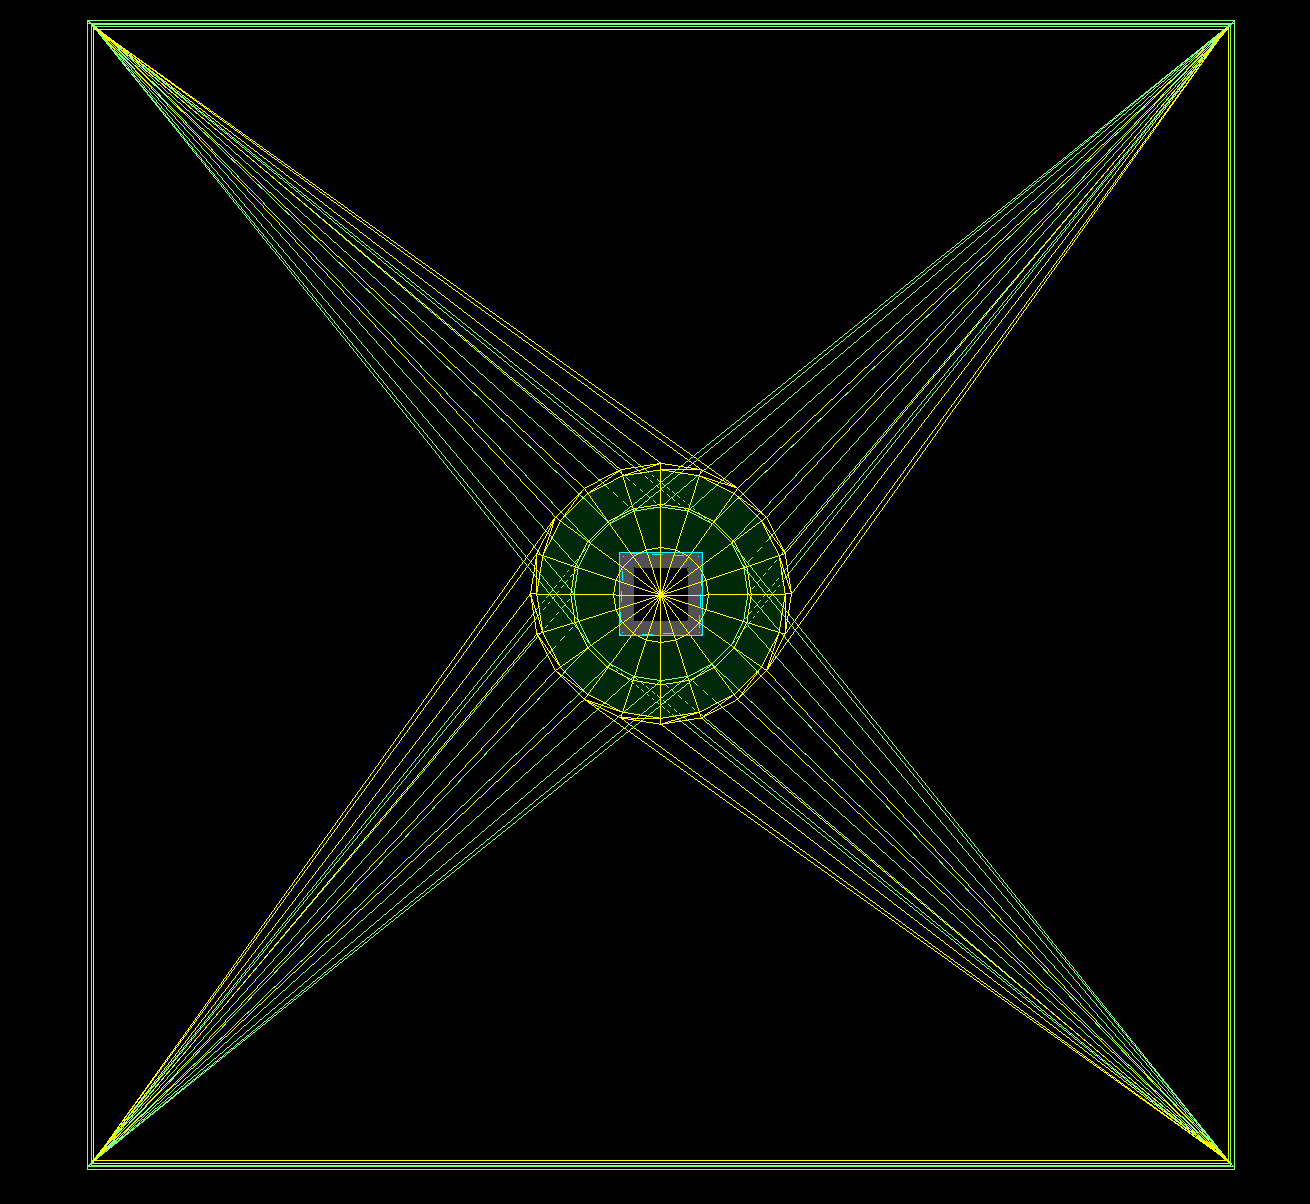
\includegraphics[width=.45\textwidth]{front.png}
%\qquad
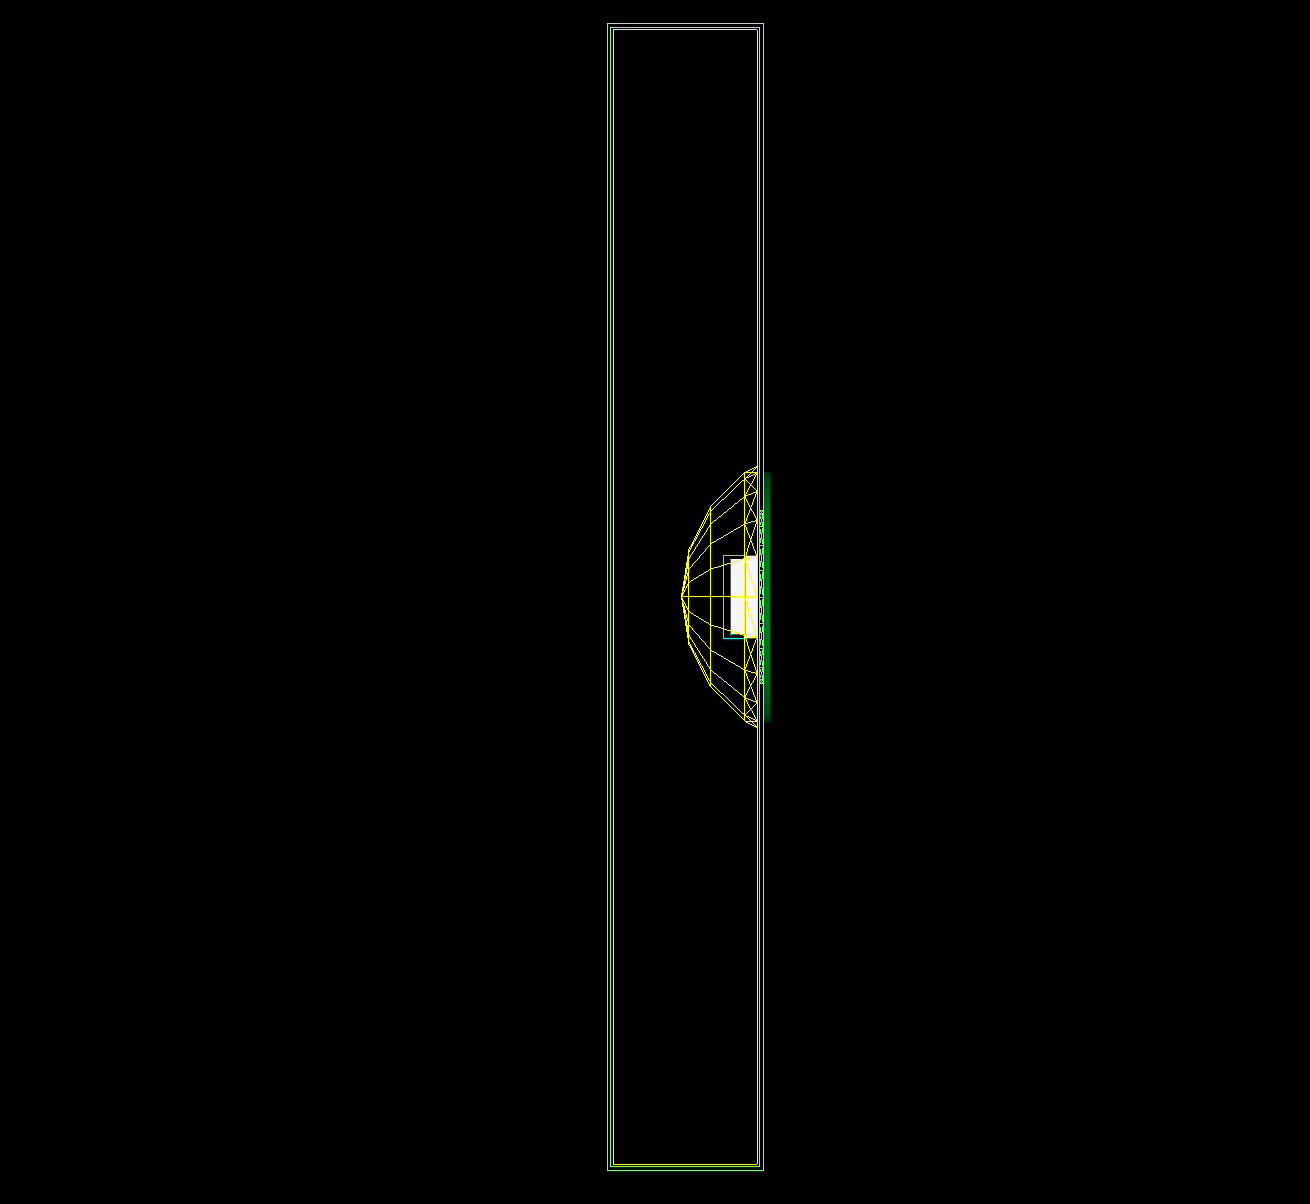
\includegraphics[width=.45\textwidth]{side.png}
% "\includegraphics" from the "graphicx" permits to crop (trim+clip)
% and rotate (angle) and image (and much more)
\caption{\label{fig:g4simu} Simulation geometry}
\end{figure}

To speed up the simulation, we start directly from photons instead of the the 120 GeV protons.
We calculated the number of photons according to the proton path length in the scintillator. 
Then, photon's starting point were set uniformly along the beam path. 
%reasons why we generate photons directly and how we managed to do that


There are several reasons why we think such a skip is acceptable. 
First of all, we care more about the detection efficiency of photons than the exact number. 
Thus, in our simulations, factors like the reflectivity of tile wrapping, tile sizes, dimple shape and sizes are more worthwhile to study.
Secondly, the thickness of tile is of several milimeters. 
Energetic protons could penetrate the tile easily and the path is more or less a straight line.
The number of photons is propotional to the energy deposition and photons are uniformly generated inside scintillator. 

%more details on the simulation
More than 95\% photons lost their energy  and are not detected when they are boucing back and forth. 
%the number should be checked, the efficiency is so low?
We also set a maximum track length so any photons with a longer track will be stopped immediately.
%how the data in following sections are calculated
To make a comparision with test beam data, we simulated the responses of various tile areas, thicknesses and dimple sizes. 
For each geometry, we select proton beam position uniformly across the tile and repeat the simulation 100 times to get a average response. 
%currently, the standard error is simply taken as uncertainties. Maybe more  sophisticated method will be used later.









\section{SiPM calibration}
\label{sec:calibration}

\section{Simulation Normalization}

\section{Scintillator response}
\subsection{cuts and LY determination ....}
\subsection{Tile uniformity}
\subsection{Tile cross sectional area}

\subsection{Tile thickness}

\subsection{Tile hole size}

\section{Summary}


\begin{thebibliography}{99}

\bibitem{a}
Apollinari G. et al., \emph{High-Luminosity Large Hadron Collider (HL-LHC): Technical Design Report V. 0.1}, CERN-2017-007-M (2017), doi:10.23731/CYRM-2017-004.

\bibitem{b}
CMS Collaboration, \emph{The Phase-2 Upgrade of the CMS Endcap Calorimeter}, CERN-LHCC-2017-023, CMS-TDR-019 (2019), https://cds.cern.ch/record/2293646.

\bibitem{geant4}
S. Agostinelli et al (GEANT4), Nucl. Instrum. Meth. A, 506: 250 (2003)


\end{thebibliography}
\end{document}
